\chapter{Método de trabajo}
\label{chap:metodo}

\drop{E}{n} este capítulo se describe la metodología de desarrollo aplicada, sus ventajas y motivo de elección. También se presenta la evolución del proyecto en base a la metodología empleada, los hitos conseguidos en cada fase, su complejidad y el tiempo empleado en cada una de ellas, detallando las iteraciones realizadas hasta conseguir la versión final del sistema.

Para finalizar, se listan y describen todas las herramientas utilizadas en el desarrollo, ya sean hardware o software.
%Igualmente se aportará información del rendimiento (profiling) del sistema en diferentes situaciones.

\section{Metodología del desarrollo}
Para la construcción de un proyecto de cierta envergadura, como es el caso de un Trabajo Fin de Grado, la aplicación de un marco de trabajo para estructurar, planificar y controlar el proceso, es esencial para desarrollar software de calidad.

Las características del proyecto, con requisitos con posibilidad de cambios y adaptaciones a lo largo de todo el proceso, el reducido «equipo de desarrollo» o la necesidad de obtener versiones incrementales que sean testeadas y validadas por el director de proyecto, hacen que la elección se decante hacia \textbf{metodologías ágiles} de desarrollo de software.

Las \textbf{metodologías ágiles} \cite{Ubeda}, utilizan prácticas adaptativas (no basadas en predicciones), iterativas, centradas en personas (clientes y desarrolladores), orientadas a entregas incrementales, con mucha comunicación y  necesitan que el cliente esté muy involucrado en el proyecto para recibir su \textit{feedback}. El \textit{feedback} continuo es indispensable para evitar que el cliente, con el software acabado, diga \textit{«es lo que pedí, pero no es lo que necesitaba»}, algo habitual cuando se utilizan métodos clásicos.

En resumen, las principales características a las que deben dar forma las metodologías ágiles son:
\begin{itemize}
\item \textbf{Incremental:} Versiones pequeñas de software, con ciclos rápidos. 
\item \textbf{Cooperativa:} Desarrolladores y cliente siempre en contacto constante.
\item \textbf{Directa:} El método es fácil de aprender, modificar y está bien documentado.
\item \textbf{Adaptativa:} Son capaces de tolerar los cambios propuestos por el cliente.
\end{itemize}
%Hay que tener en consideración la muy diferente naturaleza de los métodos ágiles. Mientras que Scrum se decanta por la gestión, otros como XP especifican las prácticas a seguir en el equipo, Pragmatic Programming da pautas para desarrollar un buen código, algunos como FDD no abarcan la totalidad del proceso de desarrollo, AgileUP surge como una versión ágil de RUP y propone EUP que es una ampliación para abarcar todo el ciclo de vida del software, etc.
\section{\textit{Scrum}}
Scrum está desarrollado para gestionar el proceso de desarrollo de sistemas aplicando ideas de flexibilidad, adaptabilidad y productividad. Sin llegar a describir ninguna técnica de desarrollo de software específica, el objetivo es definir cómo deben funcionar los miembros del equipo para que el sistema sea flexible y se adapte a condiciones altamente cambiantes.

\begin{figure}[t] 
  \centering
  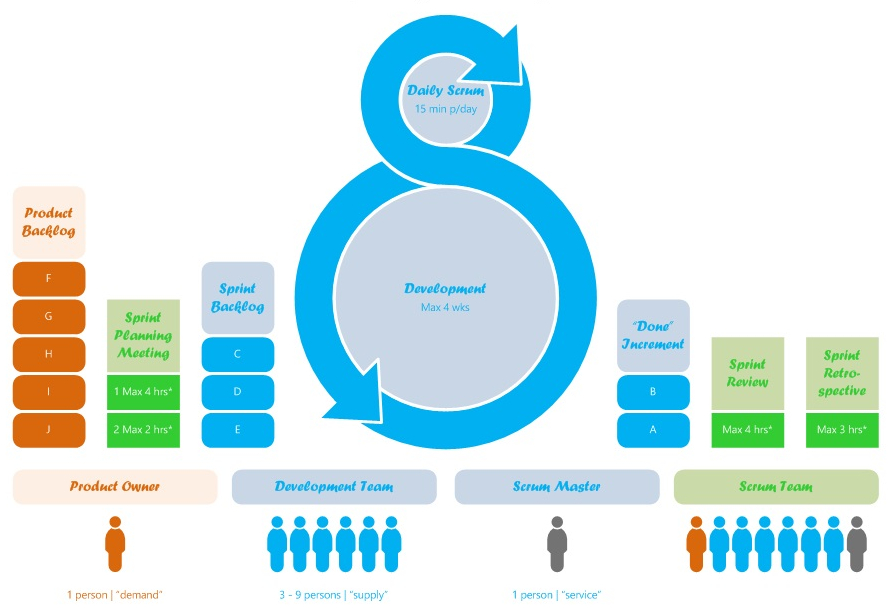
\includegraphics[width=1.0\textwidth]{scrum-overview.jpg}
  \caption{Esquema de trabajo con \textit{Scrum}. (Mark Hoogveld)}
  \label{fig:scrum}
\end{figure}

\subsection{Fases de Scrum}
El proceso de Scrum consta de tres fases: pre-game, desarrollo o game y post-game.

A continuación se detallan las fases de Scrum según Schwaber y Beedle \cite{Schwaber}. La fase pre-game incluye dos subfases:
\begin{itemize}

\item \textbf{Pre-game}
El planteamiento incluye la definición del sistema a desarrollar y asegurar la financiación. Se crea una lista de acumulación o pila de producto, \textit{product backlog list} conteniendo todos los requisitos conocidos hasta el momento. Los requisitos los puede originar el cliente, los programadores o los departamentos de ventas, marketing o atención al cliente. Se priorizan los requisitos y se estima el esfuerzo necesario para su desarrollo. La \textit{product backlog list} se actualiza constantemente con puntos nuevos y más detalles, así como con estimaciones más exactas y el nuevo orden de prioridades. El planning también incluye la definición del equipo del proyecto, herramientas y otros recursos, la valoración de riesgos, necesidades de formación y la aprobación de la gestión de comprobaciones. En cada iteración, el equipo(s) de Scrum revisa la Product Backlog list actualizada. En la jerga de Scrum, se llaman paquetes a los objetos o componentes que necesitan cambiarse en la siguiente iteración.

En la fase de la arquitectura, se crea el diseño del sistema a alto nivel basándose en los requisitos actuales del Backlog. En el caso de una mejora a un sistema ya existente, se identifican los cambios necesarios en el backlog así como los problemas que puedan causar. En una reunión se revisa el diseño del plan para cumplir las propuestas. Además, se preparan los contenidos de las versiones que serán lanzadas. 

\item \textbf{Game}
Esta fase, la parte ágil de Scrum, se trata como una caja negra donde se espera lo imprevisible. Las diferentes variables técnicas y de entorno que pueden cambiar (calendario, calidad, requisitos, recursos, tecnologías, herramientas, e incluso métodos de desarrollo) se observan y controlan durante los sprints. En lugar de considerar estos puntos sólo al principio del proyecto, Scrum los controla constantemente para adaptarse a los cambios. En la fase de desarrollo, el sistema funciona en sprints o carreras cortas. Los sprints son ciclos iterativos donde se desarrollan o mejoran las funcionalidades para producir los nuevos incrementos. Cada sprint incluye las fases habituales de desarrollo del software: requisitos, análisis, diseño, desarrollo y entrega. La arquitectura y el diseño del sistema evolucionan durante el desarrollo del sprint. Un sprint dura de una semana a un mes. Puede haber de tres a ocho sprints, por ejemplo, antes de que el sistema esté listo para lanzarse. También puede haber más de un equipo que construya cada incremento.

\item \textbf{Post-game}
Contiene el cierre de la versión. Se entra en esta fase cuando se completan todos los requisitos. En este caso, no se incorpora ni mejora ninguna función. El sistema ya está listo para lanzarse (release) y ahora se integra, se pone a prueba y se documenta.
\end{itemize}

\subsection{Roles y responsabilidades}
Los papeles en Scrum tienen tareas y propósitos diferentes durante el proceso y sus prácticas.

\begin{itemize}
\item \textbf{Scrum Master} Es responsable de asegurar que el proyecto se realiza según las prácticas, valores y reglas de Scrum y que progresa como estaba previsto. Actúa recíprocamente tanto con el equipo del proyecto como con el cliente. También es responsable de resolver cualquier impedimento para seguir trabajando tan productivamente como sea posible. 

\item \textbf{Propietario del producto} El propietario del producto es oficialmente responsable del proyecto, gestionando, controlando, y haciendo visible la Product backlog list. Es elegido por el Scrum Master, el cliente y la dirección. Toma las últimas decisiones de las tareas relacionadas con la Product backlog list, participa estimando el esfuerzo de desarrollo para los puntos del Backlog y los concreta en funcionalidades a desarrollar.

\item \textbf{Equipo de Scrum} El equipo de Scrum tiene autoridad para decidir las acciones pertinentes para organizarse y lograr lo propuesto en cada sprint. El equipo de Scrum está involucrado, por ejemplo, en estimar el esfuerzo requerido para cada parte, crear y revisar la Product Backlog list e identificar problemas a tratar.

\item \textbf{Cliente} El cliente participa en las tareas relacionadas con los puntos del Backlog para diseñar o mejorar el sistema.

\item \textbf{Director} La gestión o dirección toma la última decisión y se encarga de los documentos, normas y convenciones seguidas en el proyecto. La dirección también participa en identificar objetivos y requisitos. Por ejemplo, ayuda a seleccionar el product owner, valorar los progresos y reducir el Backlog con el Scrum Master.
\end{itemize}

\subsection{Artefactos}
\subsubsection{Documentos}
\begin{itemize}
\item \textbf{Product Backlog} El Product Backlog define todo lo necesario en el producto final, basándose en los conocimientos de ese momento. Por tanto, define el trabajo a hacer en el proyecto. Incluye una lista ordenada por prioridades y actualizada de requisitos técnicos para que el sistema se haga o mejore. Los puntos del Product Backlog, por ejemplo, pueden incluir características, funciones, parches para bugs, defectos, peticiones de mejoras o actualizaciones de tecnología.
 
También se incluyen temas que requieren solución para poder hacer otros puntos de la lista. A la lista de backlog puede contribuir el cliente, el equipo del proyecto y los departamentos de ventas, marketing y atención al cliente.
Esta práctica incluye las tareas para crear la lista de backlog, actualizarla agregando, quitando o especificando puntos con sus respectivas prioridades. El Product Owner es responsable de mantener el Product Backlog.

El Product Backlog define todo lo necesario en el producto final, basándose en los conocimientos de ese momento. Por tanto, define el trabajo a hacer en el proyecto. Incluye una lista ordenada por prioridades y actualizada de requisitos técnicos para que el sistema se haga o mejore. Los puntos del Product Backlog, por ejemplo, pueden incluir características, funciones, parches para bugs, defectos, peticiones de mejoras o actualizaciones de tecnología.
También se incluyen temas que requieren solución para poder hacer otros puntos de la lista. A la lista de backlog puede contribuir el cliente, el equipo del proyecto y los departamentos de ventas, marketing y atención al cliente.

\item \textbf{Sprint Backlog} Es el punto de partida para cada sprint, una lista de puntos de la lista del Product Backlog seleccionados para llevarse a cabo en el próximo sprint. El equipo de Scrum junto con el Scrum Master y el Product Owner seleccionan los puntos en la reunión para planear el Sprint, basándose en los puntos con prioridad y los objetivos de ese sprint. A diferencia del Product Backlog, el Sprint Backlog no se modifica hasta que el sprint (es decir, 30 días) termina.
 
Cuando todos los puntos del Sprint Backlog están completos, se prepara una nueva iteración del sistema. El registro incluye los valores que representan las horas de trabajo pendiente; en función de esos valores se acostumbra a elaborar un gráfico de quemado, usados también en muchos otros métodos.
\end{itemize}
\subsubsection{Reuniones}
\begin{itemize}
\item \textbf{Reunión diaria de Scrum} Se organizan reuniones de Scrum diarias para seguir el progreso del equipo y planear las reuniones: qué se ha hecho desde la última reunión y qué se hará para la siguiente. También se ponen sobre la mesa problemas y otros asuntos que puedan aparecer en esta reunión diaria de unos 15 minutos. Se busca y soluciona cualquier deficiencia o imprevisto del proceso. El Scrum Master dirige las reuniones. La dirección (Management), también puede colaborar en la reunión.

\item \textbf{Reunión para plantear el Sprint} El Sprint Planning meeting consta de dos fases y la organiza el Scrum Master. En la primera fase, los clientes, usuarios, la dirección, el Product Owner y el equipo, eligen los objetivos y las funcionalidades del próximo sprint. En la segunda fase, el Scrum Master y el equipo concretan la manera de conseguir esos objetivos (product increment) en el siguiente sprint.

\item \textbf{Sprint review meeting} En el último día del sprint, el equipo y el Scrum Master presentan los resultados del sprint, (el incremento producido) a la dirección, clientes, usuarios y Product Owner en una reunión informal. Los participantes evalúan la evolución y deciden sobre las siguientes actividades. La reunión de la revisión puede revelar nuevos puntos e incluso cambiar la dirección tomada del sistema que se está construyendo.

Al final de cada iteración de treinta días hay una demostración a cargo del Scrum Master. Las presentaciones en PowerPoint están prohibidas. En los encuentros diarios, todos tienen que ser puntuales; si alguien llega tarde, se le cobra una multa simbólica. Sólo se permite usar artefactos de los métodos a los que Scrum acompañe

\end{itemize}
\subsubsection{Sprint}
El sprint consiste en adaptarse a las condiciones cambiantes del proyecto como requisitos, tiempo, recursos, conocimiento, tecnología, etc. El Equipo de Scrum se organiza para producir un nuevo incremento ejecutable en un sprint que dura aproximadamente un mes natural. Las herramientas activas del equipo son las reuniones para planear el sprint, el Sprint Backlog y las reuniones diarias de Scrum.

\section{\textit{eXtreme Programming}}
\textit{Extreme Programming}  o programación extrema, surgió como respuesta a la lentitud de los modelos tradicionales de desarrollo. Los orígenes de esta metodología surgieron en 1996, cuando Kent Beck comenzó a trabajar en un proyecto para reemplazar el programa de nóminas para Chrysler. Aunque las tácticas por separado que utiliza XP no son novedosas, la manera de unirlas sí. 

En la primera edición de \textit{XP} (1999), Beck definió 4 valores, 15 principios básicos, y 12 prácticas. Posteriormente el proceso fue revisado y se publicó en 2004 \cite{Beck:2004:EPE:1076267}, en él se detallan 5 valores, 14 principios, 13 prácticas primarias y 11 prácticas secundarias.

\subsection{Valores}
\begin{itemize}
\item La mayoría de los problemas y errores provienen de la falta de comunicación. Debe haber \textbf{\textit{comunicación}} entre los miembros del equipo y entre el equipo y los clientes. La comunicación más eficaz es la comunicación directa, interpersonal. También los artefactos deben ser fácilmente entendibles y estar actualizados.

\item «Haz lo más sencillo que podría funcionar». Programar de forma sencilla, que no simplista, requiere experiencia, ideas y trabajo duro. La \textbf{\textit{simplicidad}} favorece la comunicación, reduce la cantidad de código y mejora la calidad. La idea subyacente es que las nuevas funciones se podrán agregar cuando se necesiten si el sistema es simple.

\item Siempre debería poder compararse lo que está programado con lo que se quiere programar, respecto a las funciones que se necesiten. El \textbf{\textit{feedback}} lo proporciona el contacto con el cliente y la disponibilidad de pruebas automatizadas que se desarrollan con el propio proyecto. Cuanto más simple es un sistema, más fácil es conseguir \textit{feedback} sobre él. 

\item \textbf{\textit{Valentía}}. Todos los métodos y procesos son herramientas para combatir y reducir nuestros miedos. Cuanto más miedo tengamos a un proyecto de software, mayores y más pesados serán los métodos que necesitaremos. La comunicación, la simplicidad y el feedback permiten adaptarse a los cambios grandes en los requisitos. También hay que tener valor para desechar código obsoleto.

\item Los cuatro valores anteriores implican un quinto: el \textbf{\textit{respeto}} entre los miembros y por su trabajo.
\end{itemize}

Los cinco valores no dan consejos específicos sobre cómo gestionar un proyecto, o cómo
escribir código. Para este propósito, se utilizan las prácticas que se detallan a continuación.


\subsection{Prácticas fundamentales}
– Análisis de requisitos y Planning:
\begin{itemize}
\item Se describen todas las funciones del sistema usando \textbf{historias}, descripciones breves de funciones que el cliente podrá ver.
\item El desarrollo del software se realiza \textbf{semanalmente}. Hay una reunión al principio de cada semana donde el cliente elige, según prioridades y teniendo en consideración el tiempo necesario por los programadores, las historias a programar durante la semana.
\item Evitar hacer promesas que no puedan cumplirse. 
\end{itemize}
– Equipo y Factores Humanos:
\begin{itemize}
\item Los equipos de desarrollo deben trabajar en un espacio sin divisiones para facilitar la comunicación.
\item El equipo debe componerse de miembros con todas las habilidades necesarias para el proyecto, sentido de compañerismo y de ayuda mutua. 
\item Programación por parejas. El código siempre está escrito por dos programadores en una única máquina.
\end{itemize}
– Diseño:
\begin{itemize}
\item Diseño Incremental. XP se opone a un gran diseño completo inicial (up-front). El equipo escribe código lo más pronto posible para obtener feedback y mejorar el sistema continuamente. El diseño es indispensable para obtener código bien hecho. La pregunta es cuándo diseñar. XP sugiere hacerlo incrementalmente durante la programación.
\item Primero las pruebas. Antes de actualizar y añadir código, es necesario escribir las pruebas para verificarlo. 
\end{itemize}
– Programar y lanzar versiones:
\begin{itemize}
\item El sistema debe construirse y todas las pruebas deben terminarse en diez minutos para ejecutarlo a menudo y obtener feedback. 
\item Integración continua. Los programadores deben integrar los cambios cada dos horas para evitar problemas mayores al integrar grandes partes.
\item El código y las pruebas son los únicos artefactos y se han de guardar. Los otros documentos pueden generarse a partir del código y las pruebas.
\item Cualquiera del equipo debe poder modificar cualquier parte de sistema cuando quiera. 
\item Sólo hay una versión oficial de sistema. Se puede desarrollar una rama temporal, pero sólo usarse durante unas horas.
\item Despliegue diario. Cada noche se debe poner nuevo software en producción. Es arriesgado y costoso tener diferentes versiones en producción y en el equipo.
\end{itemize}


\section{Aplicación de la metodología de desarrollo}

Para la resolución de este proyecto se ha optado por una aproximación en la que se complementan las mejores prácticas y técnicas recomendadas en \textbf{\textit{Scrum}}, con sus medidas organizativas como método de gestión y \textbf{\textit{extreme programming (XP)}}, con patrones de diseño y refactorización, como metodología de desarrollo.

%Scrum no requiere o proporciona ninguna práctica específica para el desarrollo del software. Sin embargo, se adoptarán las siguientes pautas y prácticas para evitar el caos causado por imprevistos y complejidades.
Se adoptarán las siguientes pautas y prácticas de \textbf{\textit{Scrum}} a la hora de gestionar el proceso de desarrollo:
\begin{itemize}
\item \textbf{Equipo autodirigido} y auto-organizado. 
\item Una vez elegida una tarea, \textbf{no se agrega trabajo extra}. %En caso que se agregue algo, se recomienda quitar alguna otra cosa.
\item \textbf{Iteraciones de 30 días}; se admite que sean más frecuentes.
\item \textbf{Demostración a participantes externos} al final de cada iteración. 
\item Al principio de cada iteración, \textbf{planificación adaptativa} guiada por el director.
\end{itemize}

El  equipo  de  desarrollo  lo  han constituido el autor de este TFG y Santiago Sánchez Sobrino, con  experiencia  práctica y conocimientos teóricos en metodologías ágiles. Debido  al  tamaño  del  equipo  y  condiciones  del  mismo,  las  reuniones  diarias pierden su utilidad. La figura del cliente y el director corresponde a Carlos González Morcillo, director de ambos TFG's y creador del Proyecto ARgos. 

Al comienzo de cada iteración el equipo se reunirá y creará la lista de tareas de la iteración (\textit{Sprint Backlog}) que consta de un subconjunto de las \textit{historias de usuario} de la lista de objetivos (\textit{Product Backlog}). Estas historias de usuario son seleccionadas atendiendo a las prioridades o necesidades propuestas por el Director. En esta reunión, se descompondrá cada historia en tareas, estimando el tiempo necesario para llevarlas acabo. 

Las prácticas propuestas de \textbf{\textit{XP}} que se van a utilizar son: 

\begin{itemize}
\item \textbf{Sentarse juntos.} Todo el desarrollo se llevará a cabo en un espacio que permita un trabajo cercano, cooperativo y que facilite la comunicación directa. %En las ocasiones en las que ésto no sea posible, se utilizarán medios de videoconferencia como Skype o Hangouts. 

\item \textbf{Iteraciones cortas.}  Al trabajar con pequeñas iteraciones, se obtiene el feedback del cliente con mucha frecuencia. Con esto se pretende que el producto final cubra ampliamente sus expectativas y necesidades. 

\item \textbf{Integración continua.} No se utilizarán herramientas que automaticen este proceso, no obstante, debido al tamaño reducido del equipo y a la frecuencia de las integraciones (al menos una al día), esta tarea no resultará demasiado compleja. 

\item \textbf{Diseño incremental.} A pesar de definir buena parte de la arquitectura en las primeras iteraciones, el diseño del sistema evolucionará iteración tras iteración, sometiéndose a sucesivas refactorizaciones para mejorar su calidad.  

\item \textbf{Código compartido.} Todos los miembros del equipo podrán acceder a cualquier parte del código. Sin olvidar que el presente desarrollo ágil se encuentra en el contexto de la elaboración de PFCs y que los alcances deben estar acotados para cada uno de los alumnos. Al finalizar cada  iteración se destinará tiempo a completar y refinar la documentación obtenida del proceso.

\item \textbf{Reutilización del código} Uno de los principales objetivos que se persiguen con las metodologías ágiles es entregar proyectos en tiempo y bajo presupuesto, minimizando el \textit{Time To Market}, por lo que la reutilización del código constituye un aspecto muy importante, no se ha de perder tiempo \textit{«reinventando la rueda»} en cada proyecto. Se deben obtener diseños con una alta modularidad y lo más desacoplados posibles, reutilizando como cajas negras, los elementos software que necesitemos. 

%Se ha de tener en cuenta que no todos los elementos en un proyecto son reutilizables, puesto que es inevitable que algunos estén estrechamente ligados a condiciones particulares propias de cada dominio de aplicación, la modularidad tampoco ha de convertirse en una obsesión que obstaculice el avance del proyecto. Recordemos que si se conoce la mejor forma de hacer algo, que así se haga, sino que se haga de la mejor forma conocida para la que se tenga tiempo. 
\end{itemize}

\section{Evolución del proyecto}
En este capítulo se presenta toda la documentación generada para gestionar este proyecto de desarrollo. Esta documentación está estructurada en ocho iteraciones, tal y como se describió en el estudio teórico de las metodologías ágiles. 

%\subsection{Concepto del software}

\subsection{Análisis preliminar de requisitos}
El objetivo de este proyecto es construir un sistema de ayuda a la gestión de documental que permita el tratamiento directo sobre documentos físicos impresos mediante el
uso de técnicas de visión por computador, síntesis visual y auditiva y técnicas de realidad aumentada

Los requisitos para el sistema serán proporcionados por Carlos González Morcillo, creador e investigador principal del proyecto; la cátedra Indra-UCLM y la fundación Adecco, como financiadores del proyecto y la asociación ASPRONA, que con su experiencia en la atención a personas con discapacidad, propondrán escenarios y funcionalidades que son de utilidad para este colectivo. 

El usuario final del sistema serán personas que necesiten soporte en la gestión documental debido a cualquier tipo de discapacidad.

\subsubsection{Características de los usuarios}
El fin de esté proyecto es construir un sistema que permita la integración laboral a personas con discapacidad. El tipo de usuarios a los que está dirigido es por tanto personas dentro de un amplio espectro de discapacidades.
Se debe proporcionar soporte a usuarios con discapacidades sensoriales (visuales y auditivas) e intelectuales.  

\subsubsection{Restricciones}

Debido a las características del sistema se deben tener en cuenta las siguiente restricciones:
\begin{itemize}
\item\textbf{Funcional en dispositivos móviles} El prototipo final se construirá sobre un dispositivos con arquitectura ARM con limitaciones de tanto en capacidad de computo como memoria. El sistema deberá estar optimizado para este tipo de dispositivos, obteniendo una respuesta fluida y en tiempo real.   
  
\item\textbf{Se debe basar en componentes de bajo coste} Para facilitar la implantación real en el entorno de trabajo, deberá funcionar con componentes de bajo coste, incorporando mecanismos de corrección de distorsión y registro 3D totalmente software.
\end{itemize}

\subsubsection{Interfaces Hardware}
\begin{itemize}
\item La implementación del sistema se realizará sobre una Raspberry Pi Modelo B de 512MB de RAM y arquitectura ARM 
\item La visualización será a través de un pico-proyector mediante conexión HDMI
\item El acceso al sistema y conexión a internet se establece por medio de cable ethernet durante el desarrollo y pruebas, siendo la conexión WiFi el tipo de conectividad final
\end{itemize}

\subsubsection{Requisitos funcionales}
\paragraph{Definidos en la línea base del proyecto}
\begin{itemize}
\item RF-001: Adquisición de imágenes mediante cámara USB
\item RF-002: Adquisición de imágenes mediante raspiCam
\item RF-003: Sistema de calibrado de cámaras
\item RF-004: Sistema de calibrado de proyectores
\item RF-005: Configuración del sistema mediante argumentos por terminal
\item RF-006: Captura de imágenes a distintas resoluciones
\item RF-007: Utilización de un fichero de vídeo como fuente de entrada
\item RF-008: Grabación de vídeo
\item RF-009: Sistema de cálculo de homografías
\end{itemize}

\paragraph{Definidos por ASPRONA}
\begin{itemize}
\item RFa-001: Realización de Videoconferencias
\item RFa-002: Mensajes en Lectura Fácil
\item RFa-003: Soporte para completar partes de trabajo
\item RFa-004: Soporte para completar formularios de protocolos de calidad
\item RFa-005: Guiado para clasificación y archivado de facturas
\item RFa-006: Entorno configurable por el usuario
\end{itemize}
\paragraph{Definidos por Indra/Adecco}
\begin{itemize}
\item RFi-001: Reconocimiento de Firmas
\end{itemize}
\subsubsection{Requisitos no funcionales}

\begin{itemize}
\item\textbf{Rendimiento:} El sistema debe funcionar de manera fluida y en tiempo real en dispositivos móviles basados en arquitectura ARM. Sólo existirá un único usuario del sistema simultáneamente y los documentos a tratar también se tratarán de uno en uno.
\item\textbf{Seguridad:} A parte de la información que se proporcione al usuario directamente, se mantendrá un log donde se registrará toda la actividad realizada en el sistema.
Debido al carácter experimental del proyecto, no se tendrán en cuenta la aplicación, por lo menos en la primera fases de desarrollo, de técnicas criptográficas para ficheros, bases de datos o comunicaciones.
\item\textbf{Fiabilidad:} Todo tipo de incidente producido en el sistema debe ser controlado y tratado. 
\item\textbf{Disponibilidad:} La disponibilidad del sistema debe ser de al menos un 99\% del tiempo que esté en ejecución. En caso de caída del sistema se deben proporcionar mecanismos automáticos para que la maquina y el sistema se reinicien y sean nuevamente operativos sin la necesidad de intervención directa del usuario,
\item\textbf{Mantenibilidad:} El desarrollo en un dispositivo tan reciente implica que se liberen con relativa frecuencia bibliotecas o controladores, en los que se corrigen bugs y/o mejoran su rendimiento. Seria recomendable hacer una revisión de los módulos actualizados antes de la instalación del sistema para valorar si es relevante el beneficio que aportan y no comprometer el la estabilidad del sistema.  
\item\textbf{Portabilidad:} El desarrollo se  realizará siguiendo estándares, tecnologías y bibliotecas libres multiplataforma, con el objetivo de que pueda ser utilizado en el mayor número de plataformas posibles tanto software como hardware.
\end{itemize}
\subsubsection{Otros requisitos}
La distribución del proyecto se realizará mediante alguna licencia libre como GPLv3, para ello se utilizarán bibliotecas compatibles con dicha licencia.


\subsection{Revisión sistemática de la bibliografía}
Como punto de partida para la elaboración del estado del arte se realizo una revisión sistemática de las diferentes técnicas para la identificación de documentos y su recuperación de una base de datos. Como resultado de esta revisión se ha podido conocer las técnicas más empleadas, así como sus ventajas e inconvenientes. 

El claro ganador es LLAH (Locally Likely Arrangement Hashing) con casi un 40\% de utilización ya sea con su implementación inicial o implementaciones optimizadas creadas para salvar las limitaciones del algoritmo original, lo que lo hace aún más potente y versatil.

Aunque los metodos basados en detección de descriptores de caracteristicas invariantes como SIFT, SURF, aparecen como muy utilizados, realmente no funcionan correctamente en identificación de documentos ya que no presentan zonas de textura y se producen repeticiones de patrones binarios (el propio texto cumple este patron). La mayoria son una variación del proceso inspirado en la metodologia de Lowe [SIFT], y en la que se obtienen buenos resultados sobre documentos semiestructurados realizando una selección de puntos extraidos y una adaptación del algoritmo RANSAC para la validación de supuestos aciertos en la comparación. El algoritmo tiene una tasa elevada de recuperación y precisión, es robusto a las deformaciones que pueda tener la imagen (perspectiva) y no necesita ningun paso previo de segmentación pero, como inconvenientes, no funciona ante grandes secciones de texto y la identificación que realiza es para obtener documentos similares (un ticket, un billete de tren,....) a la imagen utilizada como consulta.

Uno de los puntos del analisis de resultados, indica que al utilizar hardware con distinto rendimiento, es dificil tener mediciones normalizadas para todos los métodos. Como trabajo futuro se puede realizar para el gestor documental, la implementación de varios de los metodos más utilizados y ofrecer un estudio comparativo completo al ejecutarse en la misma plataforma.

Existen varias implementaciones optimizadas sobre LLAH para salvar las limitaciones iniciales del algoritmo. Sería un trabajo futuro la tarea de buscar sólo las publicaciones que se hayan hecho sobre LLAH e intentar crear una implementación conjunta  con todas las optimizaciones. 

\subsection{Diseño general}
\subsection{Iteraciones}
\subsubsection{Iteracion 0}
La iteración 0, se puede considerar la fase previa al inicio de la construcción. Con la idea definida, se adquiere un par de Raspberry Pi y se realiza una búsqueda de picoproyectores candidatos para el proyecto. 
El proyector debe tener un precio ajustado, ser lo más reducido posible, y ademas, tener una luminosidad suficiente para que las proyecciones sean visibles en estancias iluminadas.  

Elección del Proyector

Una vez recibida la raspberry se procede a la configuración del entorno de trabajo. Instalación de Raspbian, OpenCV, compiladores, editores y configuración del servicio de SSH para controlarla desde el puesto de trabajo.
18/nov - 12/dic

\subsubsection{Iteración 1}
El objetivo de esta primera iteración es obtener una arquitectura básica que iremos completando y refinando en cada una de las sucesivas iteraciones.

\begin{description}
\item [Captura de imágenes] La raspberry tiene opción de conectar una cámara USB. Se crea un módulo de captura de imagenes que soporte ambas cámaras.
\item [Detección de un folio en la imagen] Mediante segmentación de la imagen obtenida, detectamos una hoja de papel y obtenemos la posición de sus 4 esquinas.
\end{description}

Partiendo de las premisas que tiene el proyecto ARgos de ser un sistema autonomo, de inicio automático, sin dispositivos como ratones y teclados, en el que la experiencia de usuario vendra en función de lo que se vaya detectando en cada fotograma. Las limitadas capacidades de la raspberry pi y la experiencia que otros programadores han tenido a la hora de trabajar en sistemas de visión por computador en este dispositivo, no pone en alerta de que es posible que llegado un momento la alta carga de computo que tienen los procesos de visión por computador, afecten al rendimiento, y perdamos la sensación de tiempo real. Las consecuencias de esto es que sea necesario que los procesos más costosos deban ser ejecutados en otro dispositivo o computador con mejores prestaciones.  

Partiendo de las presimas anteriores, no queda otra opción de realizar una arquitectura completamente modular y con todos los subsistemas desacoplados. Una clase \emph{core} será la encargada de inicializar todos los subsistemas, establecer las comunicaciones entre ellos y ejecutar la lógica de usuario soportada dentro de un bucle infinito.

La raspberry tiene la opcion de conectar cámaras USB. Se construye un módulo de captura de vídeo, utilizando las funciones de la clase \texttt{VideoCapture} de OpenCV, que proporcione los distintos frames necesarios para dar soporte al resto de módulos del sistema. 

Mediante segmentación de la imagen obtenida, detectamos una hoja de papel y obtenemos la posición de sus 4 esquinas en píxeles de pantalla. Esta funcionalidad se encapsula dentro de la clase \texttt{PaperDetector}

Para la medida de rendimiento se implementa el cálculo de los FPS que da el sistema a la salida y que nos va a determinar si se obtienen resultados aceptables para un sistema de tiempo real.

Esta primera fase de pruebas nos pone en situación de los numerosos factores que influyen en este tipo de sistemas.

El primero de ellos es la iluminación. El tipo de luz (natural, fluorescente, incandescente,...), intensidad de la luz natural (luz por la mañana, al mediodia o por la tarde), dirección de la luz (crea sombras en uno u otro sentido), los reflejos producidos por las superficies se convierten en interferencias en forma de grandes manchas en la imagen. Incluso se han detectado variaciones en la detección al encontrase varias personas entre el sistema y una ventana.

En cuestión de rendimiento, los primeros resultados son mucho peores de lo esperado. A una resolución de 320x240 pixeles y solo realizando el proceso de captura y visualización de los frames capturados en pantalla, tenemos un lag de 2 segundos y una tasa de 2 FPS. Si estos valores son inadminisibles en un sistema en tiempo real con una arquitectura tan básica, y sin realizar ningún tipo de procesado en la imagen, cuando se tengan que realizar algun tratamiento a la imagen o realizar algun tipo de computo adicional, el sistema sera no usable, con una sensación de bloqueo del sistema para el usuario.   

Se vuelven a realizar las pruebas con otra cámara USB más moderna (Logitech S720) y afortunadamente los resultados mejoran sensiblemente, a 6 FPS y hasta 10 FPS para imágenes obtenidas en blanco y negro.  


\subsubsection{Iteración 2}
Los objetivos de esta iteración venian condicionados por los malos resultados obtenidos en el sprint anterior. Hay que conseguir mejorar enormente los resultados anteriores o la viabilidad del proyecto se verá seriamente afectada.

Con solo cambiar la cámara USB se obtuvieron grandes mejoras, por lo que la elección de la cámara era un elemento importante. Tras consultar en diversos foros especializados, se decide que la mejor opcion es utilizar la Raspberry Pi Camera Board, Esta cámara está especialmente diseñada para utilizarse en la raspberry y se conecta directamente al conector CSI de la placa mediante un cable plano flexible de 15 pines. Dispone de un sensor de 5MP de resolución y  puede llegar a grabar video a 1080p a 30 fps.

El gran inconveniente de es que la cámara no incluye drivers video4linux, por lo que cualquier biblioteca para lectura de cámaras web estandar, OpenCV incluido, no es capaz de obtener los frames producidos. Con la cámara se proporcionan 2 aplicaciones: raspivid y raspistill, para la captura de video e imágenes respectivamente.

Las aplicación utiliza la API MMAL (Multi-Media Abstraction Layer), para acceder a los datos de la cámara y transferirlos a la pantalla o codificarlo como imágenes o vídeos.

A partir del código fuente disponible de estas aplicaciones, Pierre Raufast modificó el código de estas aplicaciones, para que una vez obtenidos los datos de la cámara, utilizar el buffer de memoria para construir estructuras de tipo CvMat propias de OpenCV.

Partiendo del trabajo de Pierre, otras personas, como Chris Cummings o Rafael Muñoz Salinas, están construyendo bibliotecas en C++ para poder obtener las imagenes de la cámara en objetos compatibles con OpenCV.

Es precisamente la biblioteca de Rafael Muñoz, la que se ha utilizado a modo de drivers. 

Teniendo la cámara operativa y con un rendimiento óptimo, los siguientes elementos de esta iteración son:
\begin{description}
\item [Calibrado de la cámara] Diseñar y construir un sistema de calibrado para obtener los parametros intrínsecos de la cámara, necesarios para los cálculos posteriores de posicionamiento.
\item [Sistema básico de cálculo de homografias] Crer un sistema básico de cálculo homogŕafico necesario para la proyección de la perspectiva. En esta primera fase, los cálculos son los necesarios para realizar el registro y visualizarlo en la pantalla del ordenador.
\item [Dibujado mediante OpenCV] Se realizan una serie de funciones para dibujado mediante OpenCV para servir de modo debug ya que permite recibir una ventana con la imagen por medio de SSH.
\end{description}

Se construye un programa externo para el calibrado de la cámara basado en un patrón de tablero de ajedrez. Esta primera versión devuelve un fichero XML con los parametros intrinsecos de la cámara y los coeficientes de distorsión obtenidos pero no tiene en cuenta el error de reproyección.

Dentro del proyecto se crea la clase \texttt{Camera} encargada de leer los ficheros de calibración y almacenar los parametros propios de la cámera que serán utilizados para el cálculo de los parametros extrínsecos. 
Para el cálculo y almacenamiento de la posición de los folios respecto a la cámara se construye la clase \texttt{Paper}.
Para la iteración anterior se realizarón una serie de funciones auxiliares para dibujado de contornos, puntos y polígonos mediante OpenCV que sirvisen de soporte para el modo debug. Para la iteración actual, estas funciones se ha aumentado con dibujado de ejes de coordenadas, cubos y ortoedros para validar los cálculos de la posición y rotación de los folios. Con todas estas funciones se ha creado la clase estática \texttt{DrawCV}. 

Tras sustituir el módulo de captura con la nueva biblioteca para la raspberry camera board, se realizan de nuevo los test de rendimiento, y obtenemos casi 30 PFS, que es un buen resultado para aplicaciones en tiempo real.
Las pruebas realizadas al módulo de calculo de la posicion y rotación del papel, son satisfactorias, y se puede comprobar que el dibujado de ejes de coordenadas o distintos poliedros en el espacio 3D es correcto y perfectamente alineado con el papel. 

\subsubsection{Iteración 3}
El siguiente paso era incorporar el proyector al sistema. Acoplando la raspberry pi sobre el proyector y colocando la raspiCam junto a la lente obtenemos un conjunto compacto y reducido. El sistema se monta sobre un trípode y se coloca en dirección a la mesa.



\begin{description}
\item [Cálculo de homografias del sistema cámara-proyector] Un proyector se calibra usando los mismos algoritmos de calibración que una cámara ya que puede considerarse como una ``cámara invertida''. Sin embargo como el proyector no ve, el método no es tan directo como en el caso de una cámara.
Para la calibración de un proyector es inevitable el uso al menos de una cámara. Para calibrar un proyector, es necesario obtener un conjunto de coordenadas 3D-2D correspondientes. Las coordenadas pueden determinarse usando una cámara situada en una posición con una vista similar a la que tendria el proyector. El método consiste en proyectar con el proyector un plano de calibración y establecer la correspondencia entre lo proyectado y lo que vé la camara.
\end{description}
\subsubsection{Iteración 4}

\begin{description}
\item [Corrección de la orientación del papel] aaa
\item [Detector de documentos mediante descriptores de imagenes] Se realiza la implementación de detección de documentos mediante descriptores de imagenes. En esta fase se ha utilizado SURF.
\item [Optical Flow] Para la estimación y descripción del movimiento, se implementa Optical Flow  (Lucas-Kanade) que nos va a proporcionar herramientas para detección, segmentación y seguimiento de  objetos móviles en la escena a partir de un conjunto de imágenes. 
\end{description}

\subsubsection{Iteración 5}
\begin{description}
\item [Historico de percepciones] Al igual que en ARToolKit, se desarrolla una función de tratamiento del histórico de percepciones para estabilizar el tracking. Este histórico se implementa  almacenando las últimas 10 percepciones similares y realizando una media ponderada en la que las percepciones recientes tienen más peso que las antiguas. Para determinar si son percepciones próximas se establece un umbral. Mediante el uso de esta técnica eliminanos gran parte del efecto tembloroso en la proyección.
\item [Optimización del proceso de detección de rectangulos] Al igual que en ARToolKit, se desarrolla una función de tratamiento del histórico de percepciones para estabilizar el tracking. Este histórico se implementa  almacenando las últimas 10 percepciones similares y realizando una media ponderada en la que las percepciones recientes tienen más peso que las antiguas. Para determinar si son percepciones próximas se establece un umbral. Mediante el uso de esta técnica eliminanos gran parte del efecto tembloroso en la proyección.
\item [Obtencion de imagenes con RaspiCam y cámaraUSB] u obtener las ímagenes por medio de una raspiCam, que se conecta por directamente a un puerto de expansión de la placa.
\end{description}

\subsubsection{Iteración 6}
\begin{description}
\item [Detección de papeles con solapamiento] aaaa
\end{description}
\subsubsection{Iteración 7}
\begin{description}
\item [Reconocimiento de manos] aaaaa
\end{description}


\section{Tecnologías y herramientas utilizadas}

En esta sección se listan y detallan los recursos software y hardware empleados en la construcción de la plataforma. Además de una breve explicación del recurso, se enuncia la versión utilizada y sobre qué plataformas opera.

\subsection{Hardware}
\begin{itemize}
\item \textbf{Raspberry Pi}Como plataforma hardware del sistema se dispondrá de una placa Raspberry Pi, 
\item \textbf{Cámara USB} Logitech c500. 
\item \textbf{Raspberry Pi Camera Board} conectada a través de un cable plano de 15 pines MPI al puerto CSI (Camera Serie Interface) de la placa.
\item \textbf{Proyector portátil} 
\item \textbf{Amplificador de Audio} LM386 montado en una placa de test con un altavoz de 1W
\item \textbf{Equipo informático} para el desarrollo del proyecto. Intel Core i7-2600K 3.4 GHz 4 nucleos y dos hilos por nucleo 16 GB de RAM y Nvidia GeForce GTX 560 Ti

\end{itemize}

\subsection{Software}
A continuación se enumeran las diversas herramientas software empleadas y diferenciadas por categorías:

\subsubsection{Lenguajes de programación}
\begin{itemize}
\item \textbf{C++} - El lenguaje empleado para el desarrollo del proyecto ha sido C++ \cite{Stroustrup00}, debido a la eficiencia y velocidad de ejecución que proporciona a la hora trabajar en aplicaciones y sistemas en tiempo real. También por ser el estándar referente en bibliotecas gráficas y de visión artificial.
\end{itemize}

\subsubsection{Sistemas Operativos}
\begin{itemize}
\item \textbf{Debian} - Es una distribución de GNU/Linux desarrollada y mantenida por una comunidad de voluntarios. Es una de las famosas y un gran número de distribuciones estan basadas en ella. Para el desarrollo del proyecto se ha utilizado la versión \emph{unstable}. 

\item \textbf{Raspbian} - Es una distribución de GNU/Linux basada en Debian Wheeze especialmente diseñada y optimizada para la ejecución en la placa Raspberry Pi con  CPU ARMv6   
\end{itemize}

\subsubsection{Aplicaciones de desarrollo GNU}
\begin{itemize}
\item \textbf{GNU Emacs} - Editor y entorno de desarrollo. Se ha utilizado la generación del código fuente y la escritura de la documentación. Versión 24.3.1
\item \textbf{GNU Make} - Herramienta para la compilación incremental, con soporte multiproceso.
\item \textbf{GNU GCC} - La colección de compiladores GNU. En concreto se ha utilizado el compilador de C++ (g++) en su versión 4.5.2.
\item \textbf{GNU GDB} - Se trata del depurador por excelencia de los sistemas GNU/Linux. Se ha utilizado la versión 7.2.
\item \textbf{GNU GPROF} - Es una herramienta para hacer profiling (ver Sección 6.2) para compiladores de la familia gcc. Se ha utilizado la versión 2.21.
\item \textbf{GNU CMAKE} - Se trata de una herramienta análoga a make, aunque de más alto nivel, para la automatización de generación de código. Se ha utilizado principalmente para la compilación de la biblioteca RaspiCam. La versión de CMake es la 2.8.3. 
\end{itemize}

\subsubsection{Documentación y gráficos}
\begin{itemize}
\item \textbf{Doxygen} - Sistema de documentación de código fuente. Compatible con C++.
\item \textbf{InkScape} - Programa de edición de imágenes vectoriales.
\item \textbf{Draw.io} - Servicio web para dibujado de diagramas y gráficos vectoriales..
\item \textbf{GIMP} - Herramienta de manipulación de gráficos.
\item \textbf{LibreOffice Draw} - Potente herramienta de dibujado vectorial perteneciente a la suite ofimática LibreOffice. Utilizada para la generación de diagramas para la documentación. Versión 3.5.4.
\item \textbf{\LaTeX{}} - Es un sistema de composición de textos, orientado especialmente a la creación de libros, documentos científicos y técnicos que contengan fórmulas matemáticas. Elegido para la generación de la documentación mediante la distribución Texlive. 
\item  \textbf{esi-tfg} Clase \LaTeX{} del grupo \acs{ARCO} desarrollada por David Villa, y que proporciona una plantilla con la que se ha maquetado este documento.
\end{itemize}


\subsubsection{Bibliotecas}
\begin{itemize}
\item \textbf{OpenCV} - Biblioteca libre que proporciona funciones dirigidas principalmente para el desarrollo de aplicaciones de visión por computador en tiempo real. La versión utilizada es la 2.4.9
\item \textbf{RapidXML} - 
\item \textbf{RaspiCam} -  Es una biblioteca para la utilización de la cámara Raspberry Pi Board desarrollada en C++ por el grupo de investigación ``Aplicaciones de la Visión Artificial'' de la Universidad de Cordoba. La versión utilizada es la 0.1.1 
\end{itemize}

\subsubsection{Control de Versiones}
\begin{itemize}
\item \textbf{Git} - Sistema de control de versiones distribuido. Como repositorio central se ha utilizado la plataforma Bitbucket.
\end{itemize}
